\documentclass[a4paper,11pt]{report}
\usepackage[T1]{fontenc}
\usepackage[utf8]{inputenc}
\usepackage[polish]{babel}
\usepackage{lmodern}
\usepackage{graphicx}

\title{czas obsługi: stosu, listy}
\author{Tomasz Piotrowski 200524}

\begin{document}
\maketitle

\textbf {\Large{ Sprawozdanie z czasu działania algorytmów  obsługi stosu oraz listy. }}



\begin{figure}
  \begin{center}
  1.Sortowanie za pomoca algorytmu quicksort losowo wygenerowanych liczb. Pliki z wynikami dołaczone do sprawozdania. Z wykresu można wywnioskować że złożoność działania algorytmu jest liniowa.
  
    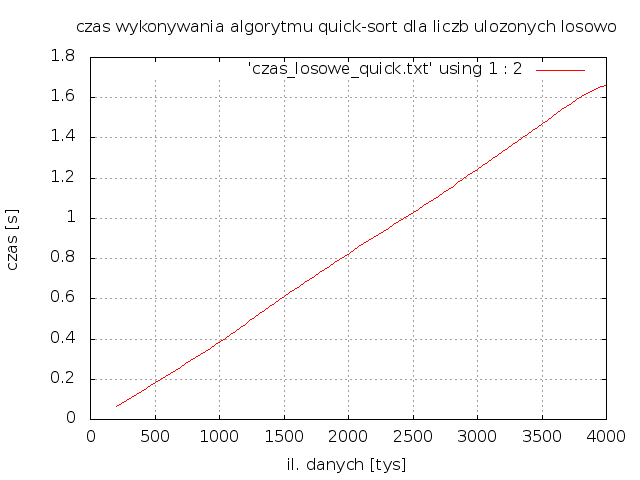
\includegraphics[scale=0.5]{./czas_losowe_quick.png}
    \label{fig:}
    \caption{}
              \begin{tabular}{|l|r|}
\hline
il[tys] & czas pół [s]  \\
\hline

200 & 0.066\\
400 & 0.148\\
600 & 0.218\\
800 &  0.298\\
1000&   0.374\\
1200&   0.464\\
1400&   0.548\\
1600&   0.696\\
1800&   0.754\\
2000&   0.81\\
2200&   0.922\\
2400&   0.982\\
2600 &  1.06\\
2800 &  1.142\\
3000 &  1.236\\
3200 &  1.354\\
3400 &  1.414\\
3600 &  1.508\\
3800 &  1.634\\
4000 &  1.66\\
\hline
\end{tabular}
\newline
  \end{center}
\end{figure}

\begin{figure}
  \begin{center}
  1.Sortowanie za pomocą algorytmu sacalania losowo wygenerowanych liczb. Pliki z wynikami dołaczone do sprawozdania. Z wykresu można wywnioskować że złożoność działania algorytmu jest liniowa.
    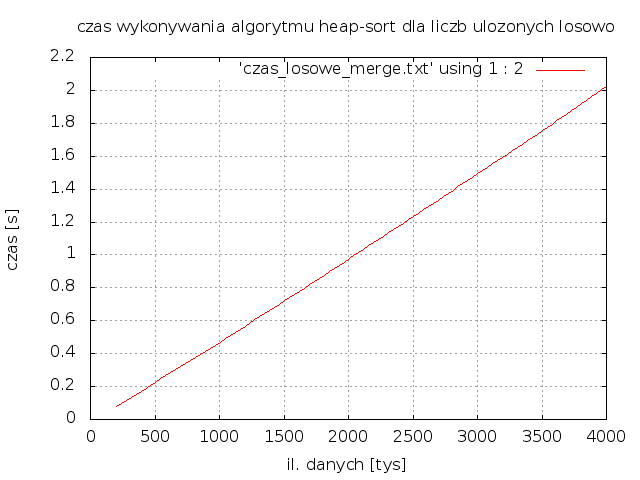
\includegraphics[scale=0.5]{./czas_losowe_merge.png}
                  \begin{tabular}{|l|r|}
\hline
il[tys] & czas pół [s]  \\
\hline
200&  0.082\\
400 & 0.176\\
600 & 0.272\\
800 & 0.368\\
1000&  0.462\\
1200&  0.566\\
1400&  0.67\\
1600 & 0.768\\
1800 & 0.862\\
2000 & 0.976\\
2200 & 1.078\\
2400 & 1.184\\
2600 & 1.278\\
2800 & 1.39\\
3000 & 1.49\\
3200 & 1.594\\
3400 & 1.704\\
3600 & 1.806\\
3800 & 1.908\\
4000 & 2.026\\
\hline
\end{tabular}
\newline
    \label{fig:}
    \caption{}
  \end{center}
\end{figure}

\begin{figure}
  \begin{center}
  1.Sortowanie za pomoca algorytmu kopcowania losowo wygenerowanych liczb. Pliki z wynikami dołaczone do sprawozdania. Z wykresu można wywnioskować że złożoność działania algorytmu jest wykładnicza.
    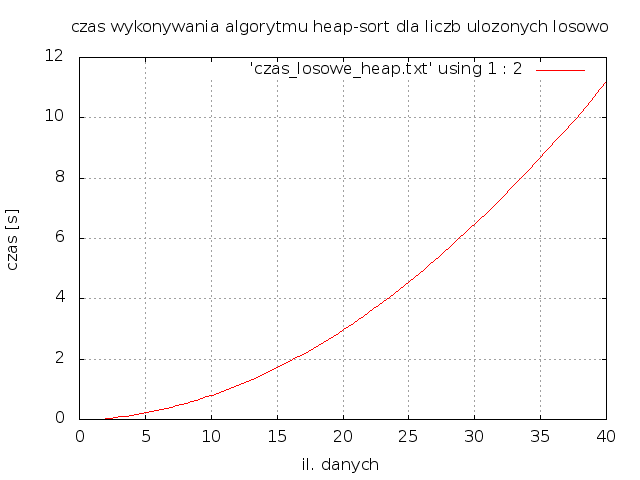
\includegraphics[scale=0.5]{./czas_losowe_heap.png}
                      \begin{tabular}{|l|r|}
\hline
il[tys] & czas pół [s]  \\
\hline
2 & 0.03\\
4 & 0.116\\
6 & 0.258\\
8 & 0.46\\
10 & 0.71\\
12 & 1.02\\
14 & 1.388\\
16 & 1.826\\
18 & 2.284\\
20 & 2.806\\
22 & 3.432\\
24 & 4.06\\
26 & 4.794\\
28 & 5.548\\
30 & 6.418\\
32 & 7.276\\
34 & 8.172\\
36 & 9.094\\
38 & 10.104\\
40 & 11.208\\
\hline
\end{tabular}
\newline
    \label{fig:}
    \caption{}
  \end{center}
\end{figure}

\begin {figure}

Testy wykazały że w przypadku losowo wygenerowanych liczb. Algorytm sortowaniea szybkiego oraz przez scalanie mają podobną złożoność obliczeniową. Jednak Algorytm sortowania szybkiego wykonał operację o 0.4s szybciej niż algorym sortowania przez scalanie. Algorytm sortowania kopcowego nadaje się do sortowania małych ilosci danych. Przewaga algorytmu sortowania kopcowego jest jego małe zapotrzebowanie na pamięć. W przypadku losowo ułożonych liczb algorytm sortowania szybkiego jest najszybszy.
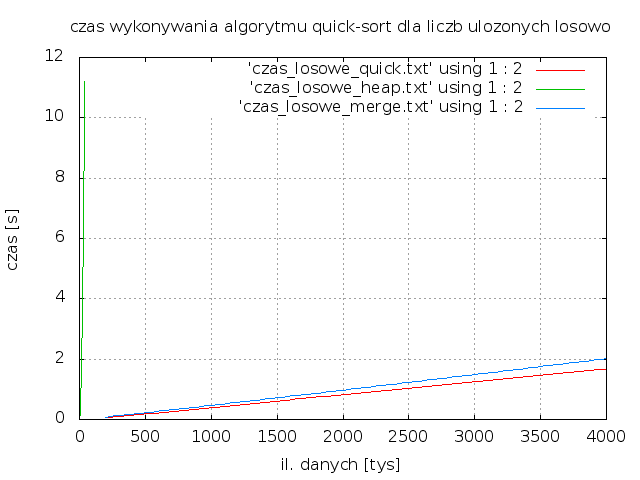
\includegraphics[scale=0.5]{./wszystkie.png}
\end{figure}

\end{document}
